\documentclass[a4paper,11pt,twoside]{report}
% THIS FILE SHOULD BE COMPILED BY pdfLaTeX

% ----------------------   PREAMBLE PART ------------------------------

% ------------------------ ENCODING & LANGUAGES ----------------------
\usepackage[utf8]{inputenc}
\usepackage[T1]{fontenc}
\usepackage[english, polish]{babel}
\usepackage{polski}
\usepackage{float}






\usepackage{amsmath, amsfonts, amsthm, latexsym} % MOSTLY MATHEMATICAL SYMBOLS

\usepackage[final]{pdfpages} % INPUTING TITLE PDF PAGE - GENERATE IT FIRST!
%\usepackage[backend=bibtex, style=verbose-trad2]{biblatex}
\usepackage{placeins}

\usepackage{commath} % various commands which can make writing math expressions easier --- documentation available at: https://ctan.gust.org.pl/tex-archive/macros/latex/contrib/commath/commath.pdf

\usepackage[hidelinks]{hyperref} % for hyperlinks, for example, urls, references to equations, entries in a bibliography --- hidelinks option removes rectangles around hiperlinks

\usepackage{caption}
\captionsetup[figure]{justification=centering, singlelinecheck=false}
\graphicspath{{../img/}}



% ---------------- MARGINS, INDENTATION, LINESPREAD ------------------

\usepackage[inner=20mm, outer=20mm, bindingoffset=10mm, top=25mm, bottom=25mm]{geometry} % MARGINS


\linespread{1.5}
\allowdisplaybreaks         % ALLOWS BREAKING PAGE IN MATH MODE

\usepackage{indentfirst}    % IT MAKES THE FIRST PARAGRAPH INDENTED; NOT NEEDED
\setlength{\parindent}{5mm} % WIDTH OF AN INDENTATION


%---------------- RUNNING HEAD - CHAPTER NAMES, PAGE NUMBERS ETC. -------------------

\usepackage{fancyhdr}
\pagestyle{fancy}
\setlength{\headheight}{14pt}
\fancyhf{}
% PAGINATION: LEFT ALIGNMENT ON EVEN PAGES, RIGHT ALIGNMENT ON ODD PAGES 
\fancyfoot[LE,RO]{\thepage} 
% RIGHT HEADER: zawartość \rightmark do lewego, wewnętrznego (marginesu) 
\fancyhead[LO]{\sc \nouppercase{\rightmark}}
% lewa pagina: zawartość \leftmark do prawego, wewnętrznego (marginesu) 
\fancyhead[RE]{\sc \leftmark}

\renewcommand{\chaptermark}[1]{\markboth{\thechapter.\ #1}{}}

% HEAD RULE - IT'S A LINE WHICH SEPARATES HEADER AND FOOTER FROM CONTENT
\renewcommand{\headrulewidth}{0 pt} % 0 MEANS NO RULE, 0.5 MEANS FINE RULE, THE BIGGER VALUE THE THICKER RULE


\fancypagestyle{plain}{
  \fancyhf{}
  \fancyfoot[LE,RO]{\thepage}
  
  \renewcommand{\headrulewidth}{0pt}
  \renewcommand{\footrulewidth}{0.0pt}
}



% --------------------------- CHAPTER HEADERS ---------------------

\usepackage{titlesec}
\titleformat{\chapter}
  {\normalfont\Large \bfseries}
  {\thechapter.}{1ex}{\Large}

\titleformat{\section}
  {\normalfont\large\bfseries}
  {\thesection.}{1ex}{}
\titlespacing{\section}{0pt}{30pt}{20pt} 

    
\titleformat{\subsection}
  {\normalfont \bfseries}
  {\thesubsection.}{1ex}{}


% ----------------------- TABLE OF CONTENTS SETUP ---------------------------

\def\cleardoublepage{\clearpage\if@twoside
\ifodd\c@page\else\hbox{}\thispagestyle{empty}\newpage
\if@twocolumn\hbox{}\newpage\fi\fi\fi}


% THIS MAKES DOTS IN TOC FOR CHAPTERS
\usepackage{etoolbox}
\makeatletter
\patchcmd{\l@chapter}
  {\hfil}
  {\leaders\hbox{\normalfont$\m@th\mkern \@dotsep mu\hbox{.}\mkern \@dotsep mu$}\hfill}
  {}{}
\makeatother

\usepackage{titletoc}
\makeatletter
\titlecontents{chapter}% <section-type>
  [0pt]% <left>
  {}% <above-code>
  {\bfseries \thecontentslabel.\quad}% <numbered-entry-format>
  {\bfseries}% <numberless-entry-format>
  {\bfseries\leaders\hbox{\normalfont$\m@th\mkern \@dotsep mu\hbox{.}\mkern \@dotsep mu$}\hfill\contentspage}% <filler-page-format>

\titlecontents{section}
  [1em]
  {}
  {\thecontentslabel.\quad}
  {}
  {\leaders\hbox{\normalfont$\m@th\mkern \@dotsep mu\hbox{.}\mkern \@dotsep mu$}\hfill\contentspage}

\titlecontents{subsection}
  [2em]
  {}
  {\thecontentslabel.\quad}
  {}
  {\leaders\hbox{\normalfont$\m@th\mkern \@dotsep mu\hbox{.}\mkern \@dotsep mu$}\hfill\contentspage}
\makeatother



% ---------------------- TABLES AD FIGURES NUMBERING ----------------------

\renewcommand*{\thetable}{\arabic{chapter}.\arabic{table}}
\renewcommand*{\thefigure}{\arabic{chapter}.\arabic{figure}}


% ------------- DEFINING ENVIRONMENTS FOR THEOREMS, DEFINITIONS ETC. ---------------

\makeatletter
\newtheoremstyle{definition}
{3ex}%                           % Space above
{3ex}%                           % Space below
{\upshape}%                      % Body font
{}%                              % Indent amount
{\bfseries}%                     % Theorem head font
{.}%                             % Punctuation after theorem head
{.5em}%                          % Space after theorem head, ' ', or \newline
{\thmname{#1}\thmnumber{ #2}\thmnote{ (#3)}}
\makeatother

\theoremstyle{definition}
\newtheorem{theorem}{Theorem}[chapter]
\newtheorem{lemma}[theorem]{Lemma}
\newtheorem{example}[theorem]{Example}
\newtheorem{proposition}[theorem]{Proposition}
\newtheorem{corollary}[theorem]{Corollary}
\newtheorem{definition}[theorem]{Definition}
\newtheorem{remark}[theorem]{Remark}

% --------------------- END OF PREAMBLE PART (MOSTLY) --------------------------





% -------------------------- USER SETTINGS ---------------------------

\newcommand{\tytul}{Badania nad technikami kompresji modeli i optymalizacji wydajności modeli głębokiego uczenia się do wdrażania na urządzeniach brzegowych}
\renewcommand{\title}{Research on Model Compression and Efficiency Optimization Techniques on Deep Learning Models for Edge Deployment}
\newcommand{\type}{Master} % Master OR Engineer
\newcommand{\supervisor}{dr inż. Promotor X} % TITLE AND NAME OF THE SUPERVISOR



\begin{document}
\raggedbottom
\sloppy
\selectlanguage{english}

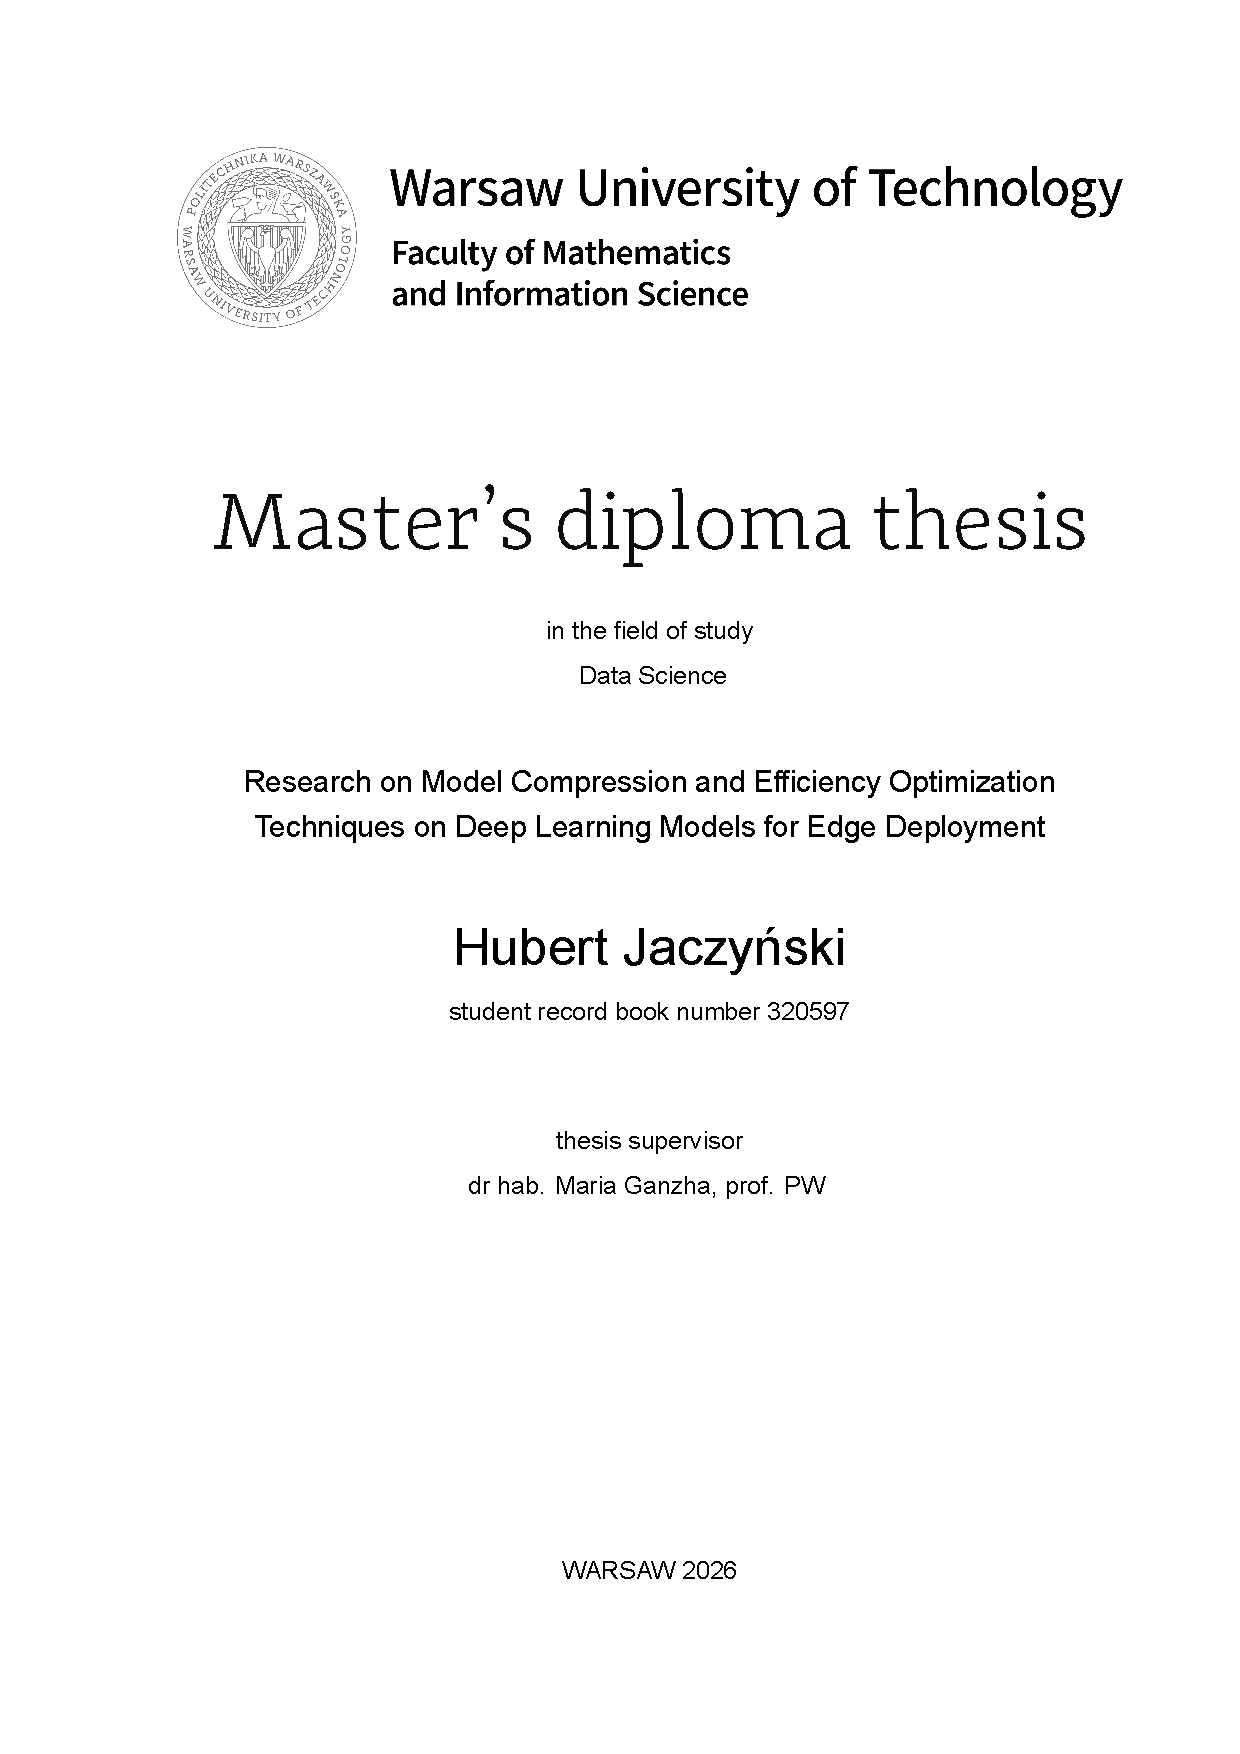
\includepdf[pages=-]{titlepage-en} % THIS INPUTS THE TITLE PAGE

\null\thispagestyle{empty}\newpage

% ------------------ PAGE WITH SIGNATURES --------------------------------

%\thispagestyle{empty}\newpage
%\null
%
%\vfill
%
%\begin{center}
%\begin{tabular}[t]{ccc}
%............................................. & \hspace*{100pt} & .............................................\\
%supervisor's signature & \hspace*{100pt} & author's signature
%\end{tabular}
%\end{center}
%


% ---------------------------- ABSTRACTS -----------------------------

{  \fontsize{12}{14} \selectfont
\begin{abstract}

\begin{center}
\title
\end{center}
Deep learning models achieve high accuracy in computer vision, but their computational and memory demands often prevent direct deployment on resource-constrained edge devices such as cameras, robots, drones, and mobile platforms. This thesis examines practical compression and acceleration techniques for modern object detectors evaluated on the COCO benchmark. The study compares three architectural families: an RF-DETR real-time detection transformer, a Swin-Transformer detector with hierarchical windowed attention, and a YOLO-style convolutional baseline. For each family, the work evaluates precision reduction, INT8 post-training quantisation, token reduction for transformer-style models, and light structured pruning. The proposed evaluation emphasises realistic deployment conditions on an NVIDIA GeForce RTX 3070 Ti and uses consistent metrics, including COCO mAP, AP@0.5, inference latency, model size, FLOPs, and, where feasible, energy-related measurements. The overall goal is to identify which techniques, and which order of applying them, provide the most favourable accuracy--latency--size trade-off for real-time object detection under limited hardware resources.

\noindent \textbf{Keywords:} Model compression, object detection, COCO, RF-DETR, Swin Transformer, YOLO, token reduction, quantisation, pruning, edge deployment
\end{abstract}
}

\null\thispagestyle{empty}\newpage


{\selectlanguage{polish} \fontsize{12}{14}\selectfont
\begin{abstract}
\begin{center}
\tytul
\end{center}
Modele głębokiego uczenia się osiągają wysoką dokładność w zakresie widzenia komputerowego, ale ich wymagania obliczeniowe i pamięciowe często uniemożliwiają bezpośrednie wdrożenie na urządzeniach brzegowych o ograniczonych zasobach, takich jak kamery, roboty, drony i platformy mobilne. Niniejsza praca bada, w jaki sposób dostosować nowoczesne modele wykrywania obiektów do wnioskowania w czasie rzeczywistym na urządzeniach, zmniejszając ich koszty obliczeniowe przy zachowaniu jakości wykrywania. W pracy dokonano przeglądu głównych rodzin architektur stosowanych w wizji (sieci konwolucyjne i modele oparte na transformatorach), a następnie skupiono się na praktycznych metodach zwiększania wydajności, które można zastosować w przypadku wdrażania na urządzeniach brzegowych. W szczególności zbadano techniki kompresji i przyspieszania modeli, w tym kwantyzację (po szkoleniu i szkolenie uwzględniające kwantyzację), przycinanie (ustrukturyzowane i nieustrukturyzowane) oraz destylację wiedzy, a także podejścia na poziomie architektury, takie jak wyszukiwanie architektury neuronowej uwzględniające sprzęt. Proponowana ocena kładzie nacisk na realistyczne warunki wdrożenia i porównuje metody przy użyciu spójnych wskaźników, w tym dokładności wykrywania, opóźnienia wnioskowania i rozmiaru modelu. Tam, gdzie to możliwe, uwzględnia również aspekty związane z energią. Ogólnym celem jest określenie, które techniki lub kombinacje technik zapewniają najkorzystniejszy kompromis między dokładnością, opóźnieniem i rozmiarem w przypadku wykrywania obiektów w czasie rzeczywistym na ograniczonym sprzęcie oraz w jakim stopniu wyniki zależą od urządzenia docelowego i czasu działania wnioskowania.

% Instead of zażółć, write:
\noindent \textbf{Słowa kluczowe:} Kompresja modeli, optymalizacja wydajności, głębokie uczenie się, sieci neuronowe, kwantyzacja, przycinanie, destylacja wiedzy, wyszukiwanie architektur neuronowych uwzględniających sprzęt, wdrażanie na urządzeniach brzegowych

\end{abstract}
}


%% --------------------------- DECLARATIONS ------------------------------------
%
%%
%%	IT IS NECESSARY OT ATTACH FILLED-OUT AUTORSHIP DEECLRATION. SCAN (IN PDF FORMAT) NEEDS TO BE PLACED IN scans FOLDER AND IT SHOULD BE CALLED, FOR EXAMPLE, DECLARATION_OF_AUTORSHIP.PDF. IF THE FILENAME OR FILEPATH IS DIFFERENT, THE FILEPATH IN THE NEXT COMMAND HAS TO BE ADJUSTED ACCORDINGLY.
%%
%%	command attacging the declarations of autorship
%%
%\includepdf[pages=-]{scans/declaration-of-autorship}
%\null\thispagestyle{empty}\newpage
%
%% optional declaration
%%
%%	command attaching the declaataration on granting a license
%%
%\includepdf[pages=-]{scans/declaration-on-granting-a-license}
%%
%%	.tex corresponding to the above PDF files are present in the 3. declarations folder 
%
\null\thispagestyle{empty}\newpage
% ------------------- TABLE OF CONTENTS ---------------------
% \selectlanguage{english} - for English
\pagenumbering{gobble}
\tableofcontents
\thispagestyle{empty}
\newpage % IF YOU HAVE EVEN QUANTITY OD PAGES OF TOC, THEN REMOVE IT OR ADD \null\newpage FOR DOUBLE BLANK PAGE BEFORE INTRODUCTION


% -------------------- THE BODY OF THE THESIS --------------------------------

\null\thispagestyle{empty}\newpage
\pagestyle{fancy}
\pagenumbering{arabic}
\setcounter{page}{11}


\chapter{Introduction}

Deep learning is used in many everyday technologies, especially in systems that analyse images and video \cite{LeCun2015DeepLearning}. The models behind these systems are improving quickly, but they are also becoming larger and more demanding to run. While powerful servers can handle such models, many real-world applications require the model to run directly on a small device, such as in cameras, robots, drones, or mobile systems \cite{Howard2017MobileNets}. These devices have limited computing power, memory, and battery capacity, so a model that performs well on a workstation may be too slow, too large, or too energy-intensive to be practical on the device \cite{Sze2017EfficientProcessing}.

For this reason, there is a growing need to make models lighter and faster while keeping their results as reliable as possible \cite{Cheng2017SurveyCompression}. In practice, this means balancing several factors: the model's accuracy, its prediction speed, the memory it requires, and the energy it consumes. The best balance depends on the intended use case — for example, a safety-critical system may prioritise accuracy, while a battery-powered device may prioritise speed and energy efficiency.

To address these challenges, researchers develop methods that reduce the computational and memory requirements of a model, while aiming to preserve performance as much as possible. Some approaches simplify the model structure, while others reduce the precision of computations, and still others transfer knowledge from a larger model to a smaller one \cite{Han2016DeepCompression}. Additionally, practical performance also depends on the specific hardware and software used to run the model, so it is essential to evaluate solutions under realistic deployment conditions \cite{Cai2019ProxylessNAS}.


\begin{figure}[H]
    \centering
        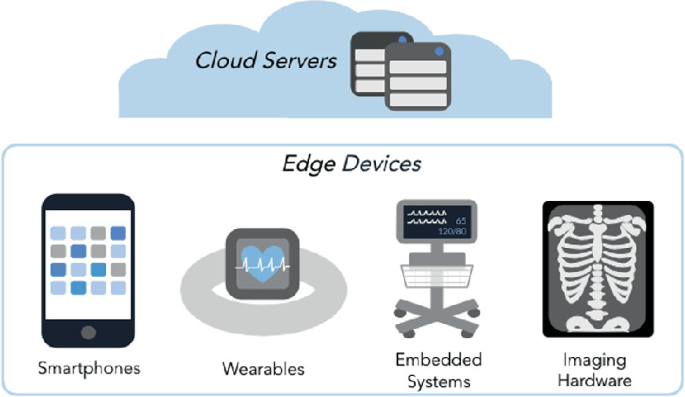
\includegraphics[width=0.8\linewidth]{edge_devices.png}
    \caption{Variants of edge devices (reproduced from \cite{Abid2022EdgeDevices}).}
    \label{fig:edge_devices}
\end{figure}


The use of these approaches may have an impact on the application of artificial intelligence in various scenarios. Some of them may not yield any benefit where the highest accuracy is required. Compression may be unacceptable without strict validation in safety-critical settings (eg. medical, automotive).

\section{Aim of the work}

This thesis focuses on real-time object detection under a constrained local hardware budget. The goal is to compare how representative detector families respond to compression and acceleration methods when evaluated on the same dataset, hardware, and measurement protocol. The work concentrates on COCO-trained detectors from three design directions: RF-DETR as a modern real-time detection transformer, Swin Transformer based detection as a hierarchical vision transformer, and YOLO-style detection as a strong convolutional baseline \cite{Robinson2025RFDETR, Liu2021Swin, UltralyticsYOLOv8}.

The experimental part will not train all detectors from scratch. Instead, it will use published COCO checkpoints and focus on evaluation, export, post-training quantisation, lightweight token reduction, and limited fine-tuning only where it is necessary to recover accuracy. This scope is suitable for a single NVIDIA GeForce RTX 3070 Ti with 8 GB of GPU memory.

The study is guided by the following research questions:

\begin{enumerate}
    \item How do RF-DETR, Swin Transformer detection, and YOLO-style detection compare on the accuracy--latency--size trade-off when evaluated under the same COCO protocol?
    \item Do token-reduction methods preserve detection accuracy better in transformer-style detectors than direct channel or filter reduction does in convolutional detectors?
    \item How much accuracy is lost, and how much latency is gained, when moving from FP32 to FP16 and INT8 post-training quantisation for each detector family?
    \item Does the order of applying compression methods matter for object detection, for example token reduction followed by INT8 quantisation versus INT8 quantisation followed by token reduction?
    \item Which compressed configurations form the best Pareto frontier for deployment on the RTX 3070 Ti, and how different are the conclusions from FLOPs-only estimates?
\end{enumerate}

The expected contribution is an empirical comparison of detector compression strategies under a reproducible local protocol, together with a discussion of which optimisation techniques are most practical for real-time edge-oriented deployment.






\chapter{Related work}
The topic addressed in this work belongs to one of the most actively researched areas in modern machine learning. As deep learning systems are deployed more widely, researchers increasingly study how far such models can be made smaller, faster, and less resource-demanding while still producing results that remain useful in practice \cite{Cheng2017SurveyCompression}. This need is driven not only by scientific interest, but also by real engineering constraints: reduced computation can lower deployment costs, enable real-time operation, and make advanced models accessible on devices with limited power, memory, and processing capability \cite{Sze2017EfficientProcessing}. At the same time, the rapid pace of technological change means that the limits of what is feasible continue to shift as new model architectures, optimisation techniques, and hardware platforms emerge \cite{Tan2020EfficientDet}.

In this thesis, artificial intelligence is considered primarily as a practical tool for automating perception tasks that would otherwise require significant human effort. Specifically, computer vision methods can be employed to detect, classify, or segment objects in images and videos \cite{Ren2015FasterRCNN, Long2015FCN}. While these tasks may appear straightforward for humans in many situations, robust performance across different environments, lighting conditions, viewpoints, and object scales remains challenging for machines. Modern deep learning approaches have achieved strong results, but they often require substantial computational resources, which motivates research on methods that reduce inference cost without sacrificing too much accuracy.

The purpose of the related works chapter is therefore to summarise the key directions of research that address efficient inference and deployment. It discusses commonly used approaches to improve efficiency, how these methods affect accuracy and runtime behaviour, and what has been reported in the literature when such techniques are applied to real-time object detection on constrained hardware \cite{Redmon2016YOLO, Han2016DeepCompression}.




\section{Neural networks}
Neural networks are inspired by the way biological nervous systems process information. In their simplest form, they consist of many small computational units (often called \emph{neurons}) that transform inputs into outputs and can be connected into larger structures. One of the earliest and most influential mathematical models of an artificial neuron was proposed by McCulloch and Pitts in 1943 \cite{McCullochPitts1943}. In this model, a neuron acts as a threshold-based logic unit: it sums its inputs and produces an output depending on whether that sum exceeds a chosen threshold \cite{McCullochPitts1943}. This idea later became a foundation for trainable models such as the perceptron and, over time, for more complex architectures \cite{Rosenblatt1958Perceptron}.

As computing power and training methods improved, neural networks evolved into many specialised families. Examples include recurrent neural networks (RNNs) for sequential data \cite{Hochreiter1997LSTM}, convolutional neural networks (CNNs) for images \cite{LeCun1998GradientBased}, generative adversarial networks (GANs) for data generation \cite{Goodfellow2014GAN}, and transformer-based models, which currently dominate many state-of-the-art results in both vision and language tasks \cite{Vaswani2017Attention}.

% \subsection{Perceptron}
% The perceptron is one of the simplest trainable neural network models \cite{Rosenblatt1958Perceptron}. It can be viewed as a single neuron that performs a weighted sum of its input features and then applies a decision function to produce a binary output. Given an input vector
% \[
% \mathbf{x} = [x_1, x_2, \dots, x_d]^T,
% \]
% The perceptron computes an activation value
% \[
% z = \mathbf{w}^T\mathbf{x} + b,
% \]
% where $\mathbf{w} = [w_1, w_2, \dots, w_d]^T$ is a vector of weights and $b$ is a bias term. The final prediction is obtained by applying a threshold function, most commonly the Heaviside step function:
% \[
% \hat{y} =
% \begin{cases}
% 1, & \text{if } z \ge 0,\\
% 0, & \text{otherwise.}
% \end{cases}
% \]

% \begin{figure}[H]
%     \centering
%     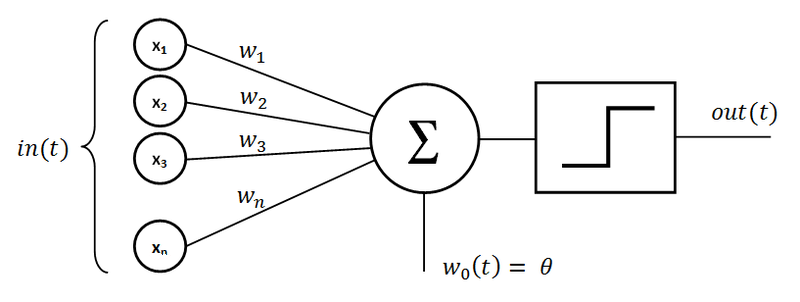
\includegraphics[width=0.8\linewidth]{Perceptron_moj.png}
%     \caption{Perceptron visualisation (reproduced from \cite{wikipedia_perceptron_pl}) (CC BY-SA 3.0).}
%     \label{fig:perceptron}
% \end{figure}


% A key feature of the perceptron is that its parameters can be learned from labelled examples \cite{Rosenblatt1958Perceptron}. For a training example $(\mathbf{x}, y)$, where $y \in \{0,1\}$ is the target label and $\hat{y}$ is the model prediction, the perceptron learning rule updates the weights as
% \[
% \mathbf{w} \leftarrow \mathbf{w} + \eta (y - \hat{y}) \mathbf{x}, \qquad
% b \leftarrow b + \eta (y - \hat{y}),
% \]
% where $\eta > 0$ is the learning rate. Intuitively, if the perceptron makes a mistake, the update shifts the decision boundary so that the current example becomes more likely to be classified correctly.

% Geometrically, the perceptron learns a linear decision boundary (a hyperplane) that separates two classes in the input space \cite{Rosenblatt1958Perceptron}. This makes it effective for \emph{linearly separable} problems. However, a single perceptron cannot solve problems that are not linearly separable, such as the classic XOR example \cite{MinskyPapert1969Perceptrons}. This limitation motivated the development of multi-layer networks, where multiple neurons are composed into deeper architectures capable of representing more complex, non-linear decision functions \cite{MinskyPapert1969Perceptrons}.



\subsection{Training neural networks}
Training a neural network means finding parameter values (weights and biases) that minimise a chosen objective function \cite{LeCun2015DeepLearning}. In supervised learning, this objective typically measures the discrepancy between the model predictions and the ground-truth labels. Let a model with parameters $\theta$ produce predictions $f(\mathbf{x};\theta)$ for an input $\mathbf{x}$. Given a dataset $\mathcal{D}=\{(\mathbf{x}_i,y_i)\}_{i=1}^{N}$ and a loss function $\ell(\cdot)$, the learning problem is commonly written as
\[
\min_{\theta}\; \mathcal{L}(\theta) 
= \frac{1}{N}\sum_{i=1}^{N} \ell\big(f(\mathbf{x}_i;\theta), y_i\big),
\]
possibly with an additional regularisation term, e.g., $\lambda \|\theta\|_2^2$, to discourage overly large weights and improve generalisation.

\subsubsection*{Gradient-based optimisation}
Modern neural networks are trained using gradient-based methods \cite{LeCun2015DeepLearning}. Gradients $\nabla_{\theta}\mathcal{L}(\theta)$ are computed efficiently with backpropagation, which applies the chain rule through the computational graph of the network \cite{Rumelhart1986Backprop}. A basic optimisation method is gradient descent, which iteratively updates parameters as
\[
\theta_{t+1} = \theta_t - \eta \nabla_{\theta}\mathcal{L}(\theta_t),
\]
where $\eta$ is the learning rate. In practice, evaluating the full gradient over all $N$ samples at every step is expensive, so training is usually performed with \emph{stochastic gradient descent} (SGD) or its variants \cite{RobbinsMonro1951}.

\subsubsection*{Stochastic gradient descent}
In SGD, the gradient is estimated using a mini-batch $\mathcal{B}_t \subset \mathcal{D}$:
\[
\theta_{t+1} = \theta_t - \eta \nabla_{\theta}\mathcal{L}_{\mathcal{B}_t}(\theta_t),
\qquad
\mathcal{L}_{\mathcal{B}_t}(\theta)=\frac{1}{|\mathcal{B}_t|}\sum_{(\mathbf{x},y)\in\mathcal{B}_t}\ell\big(f(\mathbf{x};\theta),y\big).
\]
The stochasticity introduced by mini-batches makes optimisation noisier, but also helps escape poor local regions and enables training on large datasets. Common improvements to SGD include momentum and weight decay. Momentum accumulates a running direction of descent \cite{Polyak1964}:
\[
\mathbf{v}_{t+1} = \mu \mathbf{v}_t + \nabla_{\theta}\mathcal{L}_{\mathcal{B}_t}(\theta_t),
\qquad
\theta_{t+1} = \theta_t - \eta \mathbf{v}_{t+1},
\]
where $\mu \in [0,1)$ controls how strongly past gradients influence the update.

The convergence to the minimum is shown in Figure~\ref{fig:sgd}


\begin{figure}[!htbp]
    \centering
    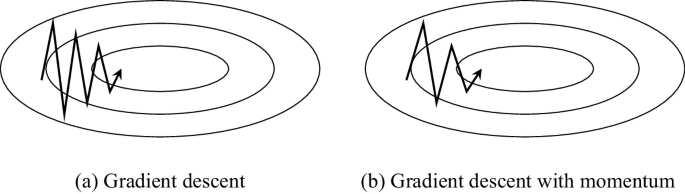
\includegraphics[width=0.8\linewidth]{SGD_with_momentum.png}
    \caption{Stochastic Gradient Descent comparison (reproduced from \cite{miller2025hmmMomentum}).}
    \label{fig:sgd}
\end{figure}


\subsubsection*{Learning rate selection and line search intuition}
The learning rate is one of the most important hyperparameters: if it is too large, the optimisation may diverge; if it is too small, convergence can be slow \cite{LeCun2015DeepLearning}. In classical optimisation, \emph{line search} methods choose a step size that sufficiently decreases the objective (for example, through the Armijo condition). Although full line search is rarely used in large-scale deep learning due to its computational cost, the same intuition is evident in practice through learning rate schedules, warm-up phases, and adaptive strategies.

A related idea is \emph{backtracking}: when an update increases the loss or causes unstable training, the step size is reduced and the update is retried. While this is not always implemented explicitly, it is conceptually similar to common training practices such as reducing the learning rate on a plateau, using gradient clipping to avoid exploding updates, or using early stopping to prevent overfitting \cite{LeCun2015DeepLearning}.

\subsubsection*{Searching for good solutions}
Neural network training is a non-convex optimisation problem, meaning there may be many parameter configurations that achieve low loss but differ in generalisation performance and robustness. As a result, training often involves a search process over:
\begin{itemize}
    \item \textbf{Optimiser choice} (e.g., SGD with momentum, Adam, AdamW),
    \item \textbf{Learning rate schedules} (step decay, cosine decay, one-cycle policy),
    \item \textbf{Regularisation} (weight decay, data augmentation, dropout),
    \item \textbf{Model capacity} (number of layers/channels, feature dimensions).
\end{itemize}
These choices influence not only final accuracy but also how well a model transfers to constrained environments, such as edge devices \cite{Sze2017EfficientProcessing}.


\section{Deep neural networks}
A deep neural network is a neural network composed of multiple successive layers, where each layer applies a learned transformation followed by a non-linear activation \cite{LeCun2015DeepLearning}. In contrast to shallow models, depth allows the network to represent complex functions through the composition of simpler operations. In computer vision, this often leads to hierarchical feature representations: early layers learn low-level patterns, such as edges and textures, while deeper layers capture higher-level structures, including object parts and entire objects \cite{LeCun2015DeepLearning}.

Despite their strong performance, deep models can be computationally demanding \cite{Sze2017EfficientProcessing}. The cost of inference is determined not only by the number of parameters (which affects storage) but also by the number of operations and the memory required to store intermediate activations. In edge deployments, limitations in processing power, memory capacity, and energy availability make these factors critical. In particular, memory access and bandwidth can become a bottleneck, meaning that reductions in model size or operation count do not always translate directly into proportional speed-ups on a given device \cite{Sze2017EfficientProcessing}.

These properties motivate the use of efficiency techniques that aim to reduce resource requirements while preserving accuracy \cite{Cheng2017SurveyCompression}. Methods such as reduced numerical precision, removal of redundant parameters or structures, transferring knowledge from larger models, and automatically searching for efficient architectures are therefore central to deploying deep networks under real-world constraints \cite{Gholami2021SurveyQuantization, Han2016DeepCompression}.


\section{Convolutional neural networks}
Convolutional Neural Networks (CNNs) are a class of deep learning models designed primarily for processing data with a grid-like structure, most notably images \cite{LeCun2015DeepLearning}. Their key idea is to exploit the spatial structure of an image by using \emph{local connectivity} and \emph{weight sharing}. Unlike fully connected layers, which learn a separate weight for every input feature, convolutional layers apply the same small set of weights (a kernel) across the entire image. This reduces the number of parameters and makes the model more efficient, while also providing a degree of \emph{translation equivariance}, meaning that shifting an object in the image results in a corresponding shift in the feature map. An example architecture is shown in Figure~\ref{fig:CNN}.

\begin{figure}[H]
    \centering
    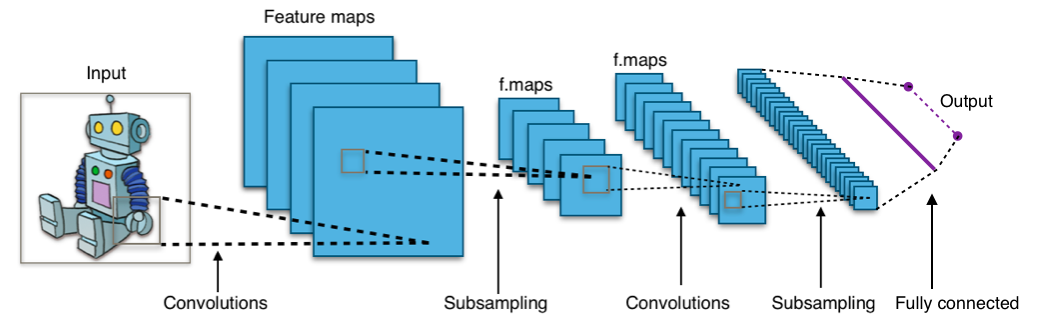
\includegraphics[width=0.8\linewidth]{Typical_cnn.png}
    \caption{CNN architecture visualisation. Reproduced from Aphex34 \cite{Aphex34_2015_TypicalCNN} (CC BY-SA 4.0).}
    \label{fig:CNN}
\end{figure}

\subsection{Convolution operation}
Given an input feature map $X \in \mathbb{R}^{H \times W \times C_{\text{in}}}$, a convolutional layer produces an output feature map $Y \in \mathbb{R}^{H' \times W' \times C_{\text{out}}}$ by sliding learnable filters over the spatial dimensions. For a filter of size $k \times k$, the output at spatial location $(u,v)$ and output channel $j$ can be written as
\begin{equation}
Y_{u,v,j} = b_j + \sum_{c=1}^{C_{\text{in}}}\sum_{p=0}^{k-1}\sum_{q=0}^{k-1}
W_{p,q,c,j}\,X_{u+p,\,v+q,\,c},
\label{eq:conv2d}
\end{equation}
where $W$ denotes the convolutional kernel weights and $b_j$ is the bias for channel $j$. In practice, convolutions often use a stride $s$ (skipping positions) and padding $P$ (extending borders) to control the spatial resolution of the output \cite{LeCun2015DeepLearning}.

Convolution is usually followed by a non-linear activation such as ReLU,
\[
\text{ReLU}(x)=\max(0,x),
\]
which enables the network to model non-linear decision functions. Stacking multiple convolutional layers allows the network to build increasingly abstract features.

\subsection{Pooling and hierarchical representations}
Many CNN architectures include pooling operations, such as max pooling, to reduce spatial resolution and increase robustness to small shifts and distortions \cite{LeCun2015DeepLearning}. For example, max pooling with window size $k \times k$ can be expressed as
\[
Y_{u,v,c} = \max_{(p,q)\in\Omega} X_{u+p,\,v+q,\,c},
\]
where $\Omega$ indexes the pooling window. Modern architectures may replace pooling with strided convolutions, but the purpose is similar: gradually reducing resolution while increasing the number of channels, forming a hierarchical representation \cite{LeCun2015DeepLearning}.

\subsection{Typical CNN building blocks}
Over time, CNNs have evolved from simple stacks of convolution and pooling layers into more advanced building blocks \cite{LeCun2015DeepLearning}:
\begin{itemize}
    \item \textbf{Residual connections} (e.g., ResNet), which add skip paths to improve gradient flow and enable deeper networks.
    \item \textbf{Normalisation layers} (e.g., Batch Normalisation), which stabilise training and often speed up convergence.
    \item \textbf{Bottleneck designs}, which use $1\times1$ convolutions to reduce and then restore channel dimensionality, decreasing computation.
\end{itemize}
These design choices are important for practical efficiency, especially when models are deployed on limited hardware \cite{Sze2017EfficientProcessing}.

\subsection{Efficiency considerations for edge deployment}
CNNs are widely used for edge inference because their operations are structured and can be implemented efficiently on GPUs, NPUs, and other accelerators \cite{Sze2017EfficientProcessing}. However, CNNs can still be computationally expensive, particularly in early layers that process high-resolution feature maps. The total inference cost is influenced by:
\begin{itemize}
    \item the input resolution $(H,W)$ and the number of channels,
    \item kernel size and stride,
    \item the number of layers and output channels,
    \item memory bandwidth required to read and write feature maps.
\end{itemize}
A common proxy for compute is the number of multiply--accumulate operations (MACs) \cite{Sze2017EfficientProcessing}. For a standard 2D convolution, the approximate MAC count is
\[
\text{MACs} \approx H'W' \cdot C_{\text{out}} \cdot (k^2 C_{\text{in}}).
\]
This expression highlights why reducing resolution, kernel size, or channel counts can strongly affect runtime \cite{Sze2017EfficientProcessing}.

\subsection{CNNs and model compression}
CNN structure makes them suitable for many compression methods discussed later in this thesis \cite{Cheng2017SurveyCompression}. For example, \emph{structured pruning} can remove entire channels or filters, directly reducing computation \cite{Han2016DeepCompression}. \emph{Quantisation} can reduce the precision of weights and activations (e.g., from FP32 to INT8), lowering memory usage and often improving latency on supported hardware \cite{Gholami2021SurveyQuantization}. Furthermore, efficient CNN variants (e.g., based on depthwise separable convolutions and other factorised operations) are often designed specifically to reduce MACs and memory access, which is particularly beneficial for real-time object detection on edge devices \cite{Howard2017MobileNets}.

Overall, CNNs remain a foundational architecture in computer vision. Even when newer paradigms, such as transformers, are used, CNN-like components are often retained in early stages or in hybrid models due to their efficiency and strong inductive bias for local spatial patterns \cite{LeCun2015DeepLearning}.



\section{Transformers}
Transformers are a class of neural network architectures originally introduced for sequence modelling tasks \cite{Vaswani2017Attention}. Their main idea is to replace recurrence with an attention mechanism that enables the model to directly relate different parts of the input to one another. This makes transformers highly parallelisable during training and enables them to capture long-range dependencies more effectively than many earlier architectures \cite{Vaswani2017Attention}.

\subsection{Self-attention mechanism}
The core component of a transformer is \emph{self-attention} \cite{Vaswani2017Attention}. Given an input sequence represented by embeddings
\[
X \in \mathbb{R}^{n \times d},
\]
where $n$ is the number of tokens and $d$ is the embedding dimension, the model computes three learned projections: queries $Q$, keys $K$, and values $V$:
\[
Q = XW_Q,\quad K = XW_K,\quad V = XW_V,
\]
where $W_Q, W_K, W_V \in \mathbb{R}^{d \times d_k}$ are trainable matrices. Attention weights are then computed using scaled dot-product attention:
\begin{equation}
\mathrm{Attention}(Q,K,V)=\mathrm{softmax}\left(\frac{QK^T}{\sqrt{d_k}}\right)V.
\label{eq:scaled_dot_product_attention}
\end{equation}
Intuitively, the softmax term determines how strongly each token should attend to all other tokens. This allows the representation of each token to be updated based on information from the entire sequence \cite{Vaswani2017Attention}.

In practice, transformers use \emph{multi-head attention}, where multiple attention operations are performed in parallel with different learned projections \cite{Vaswani2017Attention}. This enhances expressiveness by enabling the model to simultaneously focus on different types of relationships. The outputs of the heads are concatenated and projected back to the model dimension:
\[
\mathrm{MHA}(X)=\mathrm{Concat}(\mathrm{head}_1,\dots,\mathrm{head}_h)W_O.
\]

\begin{figure}[H]
    \centering
    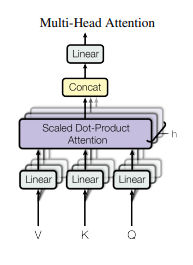
\includegraphics[width=0.5\linewidth]{Multi-Head-Attention.png}
    \caption{Multi-head attention overview (reproduced from \cite{Vaswani2017Attention}).}
    \label{fig:multi-head}
\end{figure}

\subsection{Transformer block}
A standard transformer encoder block consists of:
\begin{itemize}
    \item a multi-head self-attention layer,
    \item a position-wise feed-forward network (FFN),
    \item residual connections and normalisation layers.
\end{itemize}
A simplified formulation of an encoder block can be written as
\[
X' = \mathrm{LN}\big(X + \mathrm{MHA}(X)\big), \qquad
Y = \mathrm{LN}\big(X' + \mathrm{FFN}(X')\big),
\]
where $\mathrm{LN}(\cdot)$ denotes layer normalization. The feed-forward network is typically implemented as two linear layers with a non-linear activation:
\[
\mathrm{FFN}(x) = W_2 \sigma(W_1 x + b_1) + b_2.
\]

\begin{figure}[H]
    \centering
    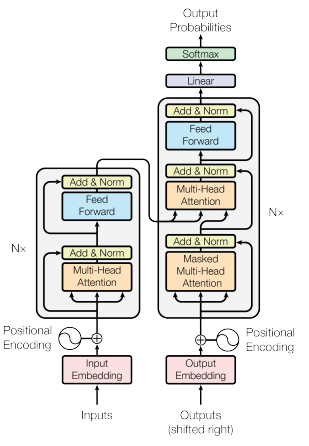
\includegraphics[width=0.5\linewidth]{transformer-architecture.png}
    \caption{Transformer architecture overview (reproduced from \cite{Vaswani2017Attention}).}
    \label{fig:transformer-architecture}
\end{figure}

\subsection{Efficiency considerations}
Compared to convolutions, the attention mechanism has a different computational profile \cite{Vaswani2017Attention}. For a sequence of length $n$, the $QK^T$ operation in Equation~\eqref{eq:scaled_dot_product_attention} has $\mathcal{O}(n^2)$ complexity, which can become expensive when $n$ is large \cite{Vaswani2017Attention}. In many practical settings, runtime and memory are influenced not only by arithmetic operations but also by the cost of moving data between memory and compute units \cite{Sze2017EfficientProcessing}. These factors are particularly important for edge deployment, where memory bandwidth and cache sizes are limited \cite{Sze2017EfficientProcessing}.

\subsection{Relation to computer vision}
Transformers were originally designed for language processing, where inputs are naturally represented as token sequences \cite{Vaswani2017Attention}. Images, however, are two-dimensional arrays of pixels. To apply transformers to vision tasks, images must be converted into a sequence representation while preserving spatial information. This motivates Vision Transformers, introduced in the next subsection \cite{Dosovitskiy2020ViT}.

\subsection{Vision Transformers}
Vision Transformers (ViTs) adapt transformer encoders to image understanding by representing an image as a sequence of fixed-size patches \cite{Dosovitskiy2020ViT}. An image of size $H \times W$ is split into patches of size $P \times P$, producing
\[
n = \frac{HW}{P^2}
\]
patches. Each patch is flattened and mapped into a $d$-dimensional embedding space. Because transformers have no inherent notion of token order, learnable \emph{positional embeddings} are added to encode patch locations \cite{Dosovitskiy2020ViT}. The resulting sequence is then processed by a standard transformer encoder stack \cite{Dosovitskiy2020ViT}.

ViTs have demonstrated strong performance, particularly when trained on large datasets, and are utilised in many modern vision systems \cite{Dosovitskiy2020ViT}. However, the quadratic cost of attention with respect to the number of patches means that high-resolution inputs can be computationally expensive \cite{Vaswani2017Attention}. As a result, many practical vision transformer variants introduce efficiency improvements, such as hierarchical token representations, local or windowed attention, and reduced token counts \cite{Liu2021Swin}. These considerations are directly relevant to edge deployment, where input resolution and model size strongly affect latency and energy consumption \cite{Sze2017EfficientProcessing}.


\section{Frugal artificial intelligence}
As deep learning systems become more widely deployed, practical limitations such as computation time, memory usage, energy consumption, and data availability increasingly determine whether a solution can be used in real-world scenarios. In many applications, especially on edge devices, it is not sufficient for a model to be accurate in a laboratory setting---it must also be efficient enough to run under strict hardware constraints and, in some cases, with limited access to training data or communication bandwidth. These constraints motivate a set of methods whose goal is to reduce the overall ``cost'' of using artificial intelligence while keeping performance as close as possible to that of unconstrained models \cite{Cheng2017SurveyCompression}.

In this thesis, the term \emph{frugal artificial intelligence} refers to the design and deployment of AI systems that aim to achieve strong predictive performance while minimising resource requirements \cite{Sze2017EfficientProcessing}. This includes reducing the computational cost of inference, lowering memory and storage demands, and improving energy efficiency \cite{Sze2017EfficientProcessing}. In addition, frugal approaches can also address data-related costs, such as the amount of labelled data needed for training or the cost of transmitting data to remote servers. The underlying idea is to build systems that are not only accurate but also feasible to deploy and maintain in environments with limited resources.

Frugal AI is particularly relevant for real-time computer vision tasks such as object detection, where models must process high-dimensional inputs (images or video frames) within strict time budgets \cite{Redmon2016YOLO}. In such settings, the core challenge is to navigate trade-offs between accuracy and efficiency. The following subsections introduce the main families of techniques used to make deep learning models more suitable for constrained deployment \cite{Cheng2017SurveyCompression}. These include reducing numerical precision, removing redundant parameters or structures, transferring knowledge from larger models to smaller ones, and automatically searching for architectures that satisfy hardware-dependent requirements \cite{Gholami2021SurveyQuantization, Hinton2015Distilling, Cai2019ProxylessNAS}.


\subsection{Quantisation}
Quantisation is a family of techniques that reduce the numerical precision used to represent a neural network. In standard deep learning workflows, model weights and activations are typically stored and computed in 32-bit floating point (FP32). Although FP32 offers high numerical accuracy, it requires significant memory bandwidth and compute \cite{Sze2017EfficientProcessing}. Quantisation replaces FP32 with lower-precision formats such as FP16 or INT8, which can reduce model size and, on supported hardware, improve inference speed and energy efficiency. This makes quantisation particularly relevant for edge deployment, where memory and power are often limited.

\subsubsection*{Basic idea}
In many practical schemes, a real-valued tensor $x$ is mapped to an integer tensor $x_q$ through an affine transformation defined by a \emph{scale} $s$ and a \emph{zero-point} $z$ \cite{Jacob2018QuantizationIntegerOnly}:
\begin{equation}
x_q = \mathrm{clip}\!\left(\left\lfloor \frac{x}{s} \right\rceil + z,\; q_{\min},\; q_{\max}\right),
\label{eq:quant_affine}
\end{equation}
where $\lfloor \cdot \rceil$ denotes rounding to the nearest integer and $[q_{\min}, q_{\max}]$ defines the representable integer range (for example $[-128,127]$ for signed INT8). During inference, values can be approximately reconstructed by
\begin{equation}
\hat{x} = s(x_q - z).
\label{eq:dequant}
\end{equation}
The parameters $s$ and $z$ are commonly derived from observed tensor ranges. If $x$ is assumed to lie in $[x_{\min},x_{\max}]$, a typical choice is
\[
s = \frac{x_{\max}-x_{\min}}{q_{\max}-q_{\min}}, 
\qquad
z = \left\lfloor q_{\min} - \frac{x_{\min}}{s} \right\rceil.
\]
This formulation is widely used in deployment toolchains because it enables efficient integer arithmetic while approximating the original floating-point computations \cite{Jacob2018QuantizationIntegerOnly}.

\subsubsection*{Weight quantisation and activation quantisation}
Quantisation can be applied to:
\begin{itemize}
    \item \textbf{Weights} (model parameters), which primarily reduces storage and improves cache efficiency. Weight-only quantisation can already provide benefits in memory-constrained scenarios.
    \item \textbf{Activations} (intermediate feature maps), which often dominate runtime memory usage during inference, especially for high-resolution vision models. Quantising activations can substantially reduce memory bandwidth requirements.
\end{itemize}
In practice, quantising activations is more challenging than quantising weights, because activation distributions depend on the input data and can vary between layers \cite{Gholami2021SurveyQuantization}.

\subsubsection*{Granularity: per-tensor vs.\ per-channel}
A key design choice is the granularity at which quantisation parameters are defined \cite{Gholami2021SurveyQuantization}:
\begin{itemize}
    \item \textbf{Per-tensor quantisation}: a single $(s,z)$ pair is used for the entire tensor. This approach is simple and efficient, but it can compromise accuracy if the ranges of different channels differ significantly.
    \item \textbf{Per-channel quantisation}: separate scales (and sometimes zero-points) are used for each output channel (common for convolution weights). This typically improves accuracy because it adapts to channel-wise variation at a small additional implementation cost.
\end{itemize}
For convolutional layers, per-channel quantisation of weights is commonly used in practice because it often yields better accuracy at the same bit-width.

\subsubsection*{Post-training quantisation (PTQ)}
Post-training quantisation converts a trained FP32 model to lower precision without re-training the model. The main advantage of PTQ is that it is fast and easy to apply. A typical PTQ workflow includes a \emph{calibration} step, where a small representative dataset is passed through the network to estimate activation ranges. PTQ is widely used in deployment scenarios when re-training is not feasible \cite{Gholami2021SurveyQuantization}.

However, PTQ may introduce a noticeable decrease in accuracy for certain models and tasks. Object detection is often more sensitive than image classification because it includes both classification and localisation components and may depend on small numerical differences in bounding box regression.

\subsubsection*{Quantisation-aware training (QAT)}
Quantisation-aware training incorporates quantisation effects during training, allowing the network to adapt to reduced precision. A common approach uses \emph{fake quantisation}: during the forward pass, tensors are quantised and dequantised to simulate INT8 behaviour, while gradients are still computed in floating-point (often using a straight-through estimator). As a result, QAT typically achieves higher accuracy than PTQ at the same bit-width, at the cost of additional training time and complexity \cite{Gholami2021SurveyQuantization}.

\subsubsection*{Symmetric vs.\ asymmetric quantisation}
Quantisation can be \cite{Gholami2021SurveyQuantization}:
\begin{itemize}
    \item \textbf{Symmetric}, where $z=0$ and the integer range is centred around zero. This can simplify computation and is common for weights.
    \item \textbf{Asymmetric}, where $z \neq 0$, allowing the range to shift. This can better represent non-zero-centred distributions and is often used for activations.
\end{itemize}
The choice affects both accuracy and hardware efficiency, and in practice, it is often determined by the deployment framework and accelerator capabilities \cite{Gholami2021SurveyQuantization}.

\subsubsection*{Why quantisation helps on edge devices}
Quantisation can improve edge inference for several reasons \cite{Sze2017EfficientProcessing}:
\begin{itemize}
    \item \textbf{Reduced model size}: fewer bits per weight lowers storage requirements and improves cache usage.
    \item \textbf{Lower memory bandwidth}: quantised activations require fewer bytes to read and write, which can be critical on constrained devices.
    \item \textbf{Faster compute on supported hardware}: many NPUs and mobile accelerators provide highly optimised INT8 operations.
    \item \textbf{Lower energy consumption}: moving and processing fewer bits often reduces power usage, which is important for battery-powered systems.
\end{itemize}
At the same time, observed speedups depend on the hardware and runtime stack. If the inference engine does not support a quantised operator, it may fall back to floating-point execution, reducing the practical benefits \cite{Sze2017EfficientProcessing}.

\subsubsection*{Quantisation in the context of compression pipelines}
Quantisation is often combined with other compression methods \cite{Cheng2017SurveyCompression}. For example, pruning can reduce the number of channels or filters, and quantisation can then further reduce memory and bandwidth \cite{Han2016DeepCompression}. Knowledge distillation can help recover accuracy lost due to low-precision constraints by training a compact quantised model to mimic a larger teacher \cite{Hinton2015Distilling}. These combinations are commonly used in edge deployment workflows because they address different sources of cost: model size, compute, and numerical precision \cite{Cheng2017SurveyCompression}.


\subsection{Pruning}
Pruning refers to a family of methods that reduce the size and computational cost of a neural network by removing parameters that are considered unnecessary \cite{Cheng2017SurveyCompression}. Modern deep learning models are often over-parameterised, meaning that they contain redundancy in their weights and internal representations. Pruning attempts to exploit this redundancy by eliminating parts of the model while maintaining accuracy as much as possible. In the context of edge deployment, pruning is attractive because it can reduce inference latency, memory usage, and energy consumption, especially when it leads to a smaller dense model that runs efficiently on standard hardware \cite{Sze2017EfficientProcessing}.

\subsubsection*{General formulation}
Let a model be parameterised by $\theta \in \mathbb{R}^n$. A common view of pruning is to introduce a binary mask $\mathbf{m} \in \{0,1\}^n$ that selects which parameters remain active:
\[
\theta' = \mathbf{m} \odot \theta,
\]
where $\odot$ denotes element-wise multiplication and $\theta'$ are the effective parameters used at inference. Pruning corresponds to setting some components of $\mathbf{m}$ to zero. The resulting pruned model is then typically fine-tuned to recover performance \cite{Han2016DeepCompression}.

\subsubsection*{Unstructured pruning}
\textbf{Unstructured pruning} removes individual weights, for example, by setting to zero weights with small magnitude \cite{Han2016DeepCompression}:
\[
m_i =
\begin{cases}
0, & \text{if } |\theta_i| < \tau,\\
1, & \text{otherwise,}
\end{cases}
\]
where $\tau$ is a threshold chosen to reach a desired sparsity level. This approach can substantially reduce the number of non-zero parameters, but the remaining weights form irregular sparse patterns. In practice, unstructured sparsity does not always translate into lower latency on edge devices because efficient execution often requires specialised sparse kernels or hardware support. Without such support, a sparse model may be stored compactly but still executed as if it were dense \cite{Sze2017EfficientProcessing}.

\subsubsection*{Structured pruning}
\textbf{Structured pruning} removes whole structures such as convolutional channels, filters, attention heads, or complete blocks. This produces a smaller dense network with reduced tensor dimensions, which typically provides more predictable speedups on common accelerators \cite{Sze2017EfficientProcessing}.

For example, in a convolutional layer, one may prune output channels (filters). If the original convolution has $C_{\text{out}}$ output channels, pruning removes a subset of these channels and adjusts subsequent layers accordingly. This directly reduces both parameter count and computational cost, since the approximate MAC count of a convolution scales with channel dimensions:
\[
\text{MACs} \approx H'W' \cdot C_{\text{out}} \cdot (k^2 C_{\text{in}}).
\]
Reducing $C_{\text{out}}$ (and often $C_{\text{in}}$ in downstream layers) therefore reduces compute and memory traffic \cite{Sze2017EfficientProcessing}.

\subsubsection*{Pruning criteria}
Pruning methods differ mainly in how they decide what to remove. Common criteria include~\cite{Cheng2017SurveyCompression}:
\begin{itemize}
    \item \textbf{Magnitude-based pruning}: removes weights or channels with small magnitude (simple and widely used).
    \item \textbf{Gradient-based or sensitivity-based pruning}: removes parameters that have a small effect on the loss, often estimated using gradients or second-order approximations.
    \item \textbf{Norm-based channel pruning}: removes channels with small $\ell_1$ or $\ell_2$ norm in convolution kernels.
\end{itemize}
In practice, magnitude- or norm-based pruning is popular because it is easy to implement and often provides a good baseline.

\subsubsection*{One-shot vs.\ iterative pruning}
Pruning can be applied:
\begin{itemize}
    \item \textbf{One-shot}, where a fixed fraction of parameters is removed at once, followed by fine-tuning.
    \item \textbf{Iteratively}, where pruning is performed gradually over multiple stages (e.g., prune a small fraction, fine-tune, repeat). This often yields better accuracy for the same final sparsity because the network has time to adapt \cite{Han2016DeepCompression}.
\end{itemize}
Iterative pruning is especially common when aggressive compression is required, such as for real-time inference on constrained devices.

\subsubsection*{Pruning and fine-tuning}
After pruning, fine-tuning is usually required \cite{Han2016DeepCompression}. Pruning changes the model capacity and can disrupt learned representations. Fine-tuning allows the remaining parameters to adapt and compensate for removed components. In some workflows, pruning is integrated into training by adding sparsity-inducing regularisation, for example, an $\ell_1$ penalty on weights or structured regularisers that encourage entire channels to become small.

\subsubsection*{Pruning for edge deployment}
For edge deployment, the practical benefit of pruning depends strongly on whether pruning reduces the \emph{actual} runtime bottlenecks \cite{Sze2017EfficientProcessing}. Structured pruning typically provides more consistent improvements because it reduces tensor sizes and can be accelerated by standard dense kernels. In contrast, unstructured pruning may yield a smaller parameter count without latency gains unless the target device and inference engine support sparse computation \cite{Sze2017EfficientProcessing}.

When applied to object detection models, pruning must be performed carefully because detection performance can be sensitive to capacity reductions, especially for small objects and complex scenes \cite{Cheng2017SurveyCompression}. Common practice is to primarily prune the backbone and neck components (which dominate computation) while preserving critical parts of the detection head. In many cases, pruning is combined with other methods such as quantisation or knowledge distillation to recover accuracy while maintaining a smaller and faster model.



\subsection{Knowledge distillation}
Knowledge distillation is a training strategy used to improve the performance of a compact model by transferring information from a larger, typically more accurate model. The larger model is referred to as the \emph{teacher}, while the smaller model is the \emph{student}. The primary motivation is that small models often have limited capacity and may struggle to achieve high accuracy when trained solely with hard ground-truth labels. A teacher model can provide richer supervision signals that help the student learn a better decision function without increasing inference cost \cite{Hinton2015Distilling}.

\subsubsection*{Teacher--student framework}
In the teacher--student setup, the teacher network $f_T(\cdot)$ is trained first (or chosen as an already strong model). The student network $f_S(\cdot)$ is then trained using both:
\begin{itemize}
    \item \textbf{hard labels} (the original targets), and
    \item \textbf{soft targets} derived from the teacher outputs.
\end{itemize}
Soft targets contain information about class similarities and uncertainties. For example, if the teacher assigns non-zero probability to multiple classes, it communicates that these classes are visually related, which can improve generalisation compared to training only on one-hot labels \cite{Hinton2015Distilling}.

\subsubsection*{Logit distillation and temperature scaling}
A common form of distillation uses the teacher and student logits (pre-softmax outputs). Let $\mathbf{z}_T$ and $\mathbf{z}_S$ denote teacher and student logits for the same input. Their softened probability distributions are computed with a temperature parameter $\tau > 1$:
\begin{equation}
p_T(\tau) = \mathrm{softmax}\!\left(\frac{\mathbf{z}_T}{\tau}\right),
\qquad
p_S(\tau) = \mathrm{softmax}\!\left(\frac{\mathbf{z}_S}{\tau}\right).
\label{eq:kd_softmax_temp}
\end{equation}
Higher $\tau$ produces a softer distribution, revealing more information about the teacher's relative preferences among classes. The student is trained by minimising a weighted combination of the standard supervised loss and the distillation loss:
\begin{equation}
\mathcal{L} = (1-\lambda)\,\mathcal{L}_{\text{sup}}(y, p_S(1))
+ \lambda\,\tau^2\,\mathrm{KL}\!\big(p_T(\tau)\,\|\,p_S(\tau)\big),
\label{eq:kd_loss}
\end{equation}
where $\lambda \in [0,1]$ balances the two objectives, and $\mathrm{KL}(\cdot\|\cdot)$ is the Kullback--Leibler divergence. The $\tau^2$ term is commonly used to maintain comparable gradient magnitudes across different temperature choices \cite{Hinton2015Distilling}.

\subsubsection*{Distillation beyond logits}
While logit distillation is widely used for classification, distillation can also transfer information from intermediate representations. Common extensions include:
\begin{itemize}
    \item \textbf{Feature distillation}: the student is encouraged to match the teacher's feature maps at selected layers.
    \item \textbf{Attention distillation}: the student matches attention maps or activation patterns, which can guide where the model should focus.
    \item \textbf{Relation distillation}: the student learns relationships between samples or regions that are captured by the teacher.
\end{itemize}
These variants can be particularly helpful when the student architecture differs significantly from the teacher \cite{Hinton2015Distilling}.

\subsubsection*{Knowledge distillation for object detection}
Object detection is more complex than classification because the model must solve multiple sub-tasks, typically including classification and localisation of bounding boxes. As a result, distillation for detection often combines multiple signals, such as:
\begin{itemize}
    \item distillation of classification scores,
    \item distillation of bounding box regression outputs,
    \item distillation of intermediate features (e.g., backbone or neck feature maps),
    \item distillation of region-level predictions (for two-stage detectors) or dense prediction maps (for one-stage detectors).
\end{itemize}
Because the output structure is richer, detection distillation methods must be designed carefully to avoid transferring teacher errors or overly constraining the student \cite{Ren2015FasterRCNN}.

\subsubsection*{Why distillation is useful for compression}
Distillation is especially useful in compression pipelines because it can reduce the accuracy gap between a compact model and a large baseline without increasing inference cost \cite{Cheng2017SurveyCompression}. This makes it complementary to other efficiency methods:
\begin{itemize}
    \item A \textbf{pruned} model can be fine-tuned with distillation to recover performance lost by removing channels or filters.
    \item A \textbf{quantised} model can be trained with distillation so that reduced precision causes smaller accuracy degradation.
    \item A \textbf{lightweight student architecture} (manually designed or found by NAS) can be distilled from a stronger teacher to improve accuracy under strict latency or energy constraints.
\end{itemize}
In edge deployment scenarios, where model capacity is limited, distillation is often one of the most effective ways to maintain accuracy while meeting runtime budgets \cite{Sze2017EfficientProcessing}.

\subsubsection*{Limitations and practical considerations}
Although distillation can significantly improve compact models, it also introduces additional training complexity \cite{Hinton2015Distilling}. A strong teacher is required, and the choice of distillation targets, temperature $\tau$, and weighting $\lambda$ can influence results. Moreover, the student may inherit some of the teacher's biases or failure modes. For these reasons, distillation is typically evaluated in conjunction with other compression techniques under consistent deployment conditions \cite{Cheng2017SurveyCompression}.


\subsection{Neural Architecture Search and Hardware-aware design}
Neural Architecture Search (NAS) is a family of methods that automate the design of neural network architectures \cite{Cai2019ProxylessNAS}. Instead of manually choosing the number of layers, channel widths, kernel sizes, or attention configurations, NAS explores a predefined \emph{search space} of candidate architectures and aims to identify models that achieve strong performance. This approach is particularly relevant in the context of efficient deployment, because the architecture itself strongly influences inference latency, memory usage, and energy consumption \cite{Sze2017EfficientProcessing}.

\subsubsection*{Problem formulation}
NAS can be expressed as an optimisation problem over architectures $\alpha$ from a search space $\mathcal{A}$. The goal is often to maximise predictive performance while satisfying efficiency constraints:
\begin{equation}
\max_{\alpha \in \mathcal{A}} \; \mathrm{Acc}(\alpha)
\quad \text{subject to} \quad
\mathrm{Cost}(\alpha) \le C_{\max},
\label{eq:nas_constraint}
\end{equation}
where $\mathrm{Cost}(\alpha)$ can represent latency, parameter count, memory usage, energy consumption, or a combination of these metrics. In many edge scenarios, the constraint is expressed directly as a latency budget measured on a target device \cite{Cai2019ProxylessNAS}.

Alternatively, the objective may be written as a multi-objective trade-off, for example maximising accuracy while penalising cost:
\[
\max_{\alpha \in \mathcal{A}} \; \mathrm{Acc}(\alpha) - \beta\,\mathrm{Cost}(\alpha),
\]
where $\beta$ controls how strongly efficiency is prioritised.

\subsubsection*{Search strategies}
NAS approaches differ mainly in the strategy used to explore the search space. Common strategies include:
\begin{itemize}
    \item \textbf{Evolutionary search}, where architectures are mutated and selected over generations.
    \item \textbf{Reinforcement learning}, where a controller proposes architectures and receives rewards based on performance.
    \item \textbf{Gradient-based NAS}, where a continuous relaxation of the search space allows optimisation by gradient descent.
\end{itemize}
In addition to the search strategy, NAS also depends on how candidate architectures are evaluated, which is often the dominant computational cost \cite{Cai2019ProxylessNAS}.

\subsubsection*{Hardware-aware design}
In practice, theoretical measures such as FLOPs do not always predict real latency on a specific device. Hardware-aware methods, therefore, incorporate device-dependent measurements or predictors. A hardware-aware formulation replaces $\mathrm{Cost}(\alpha)$ with a metric measured on a target platform (or estimated by a surrogate model):
\[
\mathrm{Cost}(\alpha) = \mathrm{Lat}_{\text{device}}(\alpha) \quad \text{or} \quad \widehat{\mathrm{Lat}}_{\text{device}}(\alpha).
\]
This is important because practical runtime is influenced by factors such as memory bandwidth, kernel implementations, operator fusion, and the inference engine \cite{Sze2017EfficientProcessing}. For edge deployment, hardware-aware NAS can therefore produce architectures that are efficient \emph{in practice}, not only on paper.

\subsubsection*{Computational requirements and practical limitations}
A major drawback of NAS is its computational cost. Evaluating many candidate architectures can require significant resources, often involving repeated training or fine-tuning. Early NAS approaches were prohibitively expensive, sometimes requiring hundreds or thousands of GPU-days. Although modern methods have improved efficiency (e.g., weight sharing, early stopping, or proxy tasks), NAS can still be difficult to perform under limited computational budgets \cite{Cai2019ProxylessNAS}.

For this reason, when compute resources are constrained, NAS is often used in a reduced or practical form, for example:
\begin{itemize}
    \item restricting the search space to a small set of design choices,
    \item using pre-trained backbones and searching only parts of the network (e.g., detection head or neck),
    \item relying on published efficient architectures as baselines rather than performing a full search \cite{Tan2020EfficientDet}.
    \item using lightweight proxy metrics or latency predictors instead of measuring every candidate on hardware.
\end{itemize}
These strategies allow some benefits of architecture optimisation without the full computational cost of large-scale NAS \cite{Cai2019ProxylessNAS}.

\subsubsection*{Relation to model compression}
NAS and compression address efficiency in complementary ways. Compression methods such as pruning and quantisation start from an existing architecture and aim to reduce its cost after training \cite{Cheng2017SurveyCompression}. NAS, in contrast, aims to discover architectures that are efficient \emph{by design} \cite{Cai2019ProxylessNAS}. In practice, both approaches can be combined: an architecture designed or selected for efficiency may still benefit from pruning, quantisation, or distillation to further meet strict edge constraints. From an edge deployment perspective, this combination is often attractive because it balances model quality with practical runtime performance \cite{Sze2017EfficientProcessing}.

\section*{Summary}
This chapter introduced the core building blocks used throughout the thesis: neural networks and their training, convolutional networks for vision workloads, and transformer-based models, including vision transformers, as modern alternatives for sequence-style processing in vision \cite{LeCun2015DeepLearning, Vaswani2017Attention, Dosovitskiy2020ViT}.

It then motivated \emph{frugal artificial intelligence} as a practical viewpoint where accuracy must be balanced against latency, memory, energy, and data/communication constraints typical of edge deployment \cite{Sze2017EfficientProcessing}. To meet these constraints, the chapter reviewed four main families of efficiency methods: quantisation (lower numerical precision), pruning (removing parameters/structures), knowledge distillation (teacher--student transfer), and hardware-aware NAS (architectures optimised under device-specific cost metrics). Finally, it highlighted that real deployment performance depends on the full hardware--software stack (e.g., operator support, memory bandwidth, runtime kernels), so evaluation should reflect realistic conditions rather than relying only on proxy metrics.


\chapter{Experimental methodology}

This chapter defines the experimental plan used to compare model compression strategies for object detection. The central idea is to evaluate a small but representative set of COCO-trained detectors under a shared protocol, then measure how accuracy and runtime change after applying progressively stronger efficiency methods. The study uses COCO because it is a standard object detection benchmark with established evaluation metrics and public checkpoints \cite{Lin2014COCO}.

\section{Hardware and practical scope}

The local experimental device is an NVIDIA GeForce RTX 3070 Ti with 8 GB of GPU memory. This hardware is powerful enough for inference benchmarking, export experiments, calibration, and short fine-tuning runs, but it is not appropriate for training large COCO detectors from scratch. Therefore, the experimental scope is deliberately focused on:

\begin{itemize}
    \item COCO validation-set evaluation of published checkpoints,
    \item FP32 and FP16 inference on the local GPU,
    \item INT8 post-training quantisation using a representative calibration subset,
    \item token reduction in transformer-style models,
    \item light structured pruning with limited fine-tuning when memory permits.
\end{itemize}

Batch size 1 is the primary latency setting because it corresponds to real-time camera-like inference. Batch size 8 is treated as a secondary throughput setting and may be skipped for the largest variants if memory usage becomes unstable.

\section{Candidate detector families}

The study compares three detector families that cover different architectural assumptions:

\begin{table}[H]
\centering
\small
\begin{tabular}{p{0.22\linewidth} p{0.28\linewidth} p{0.38\linewidth}}
\hline
Family & Candidate model & Reason for inclusion \\
\hline
Real-time DETR & RF-DETR Nano/Medium & Detection transformer designed for strong COCO accuracy--latency trade-offs and released with ready COCO checkpoints \cite{Robinson2025RFDETR}. \\
Hierarchical ViT & Swin-T Mask R-CNN & Windowed hierarchical transformer detector with public MMDetection configs and COCO checkpoints \cite{Liu2021Swin}. \\
CNN/YOLO baseline & YOLOv8s or YOLOv8m & Dense convolutional one-stage detector with widely used COCO checkpoints and simple export/benchmark tooling \cite{UltralyticsYOLOv8}. \\
\hline
\end{tabular}
\caption{Detector families selected for the experimental comparison.}
\label{tab:detector_families}
\end{table}

RF-DETR Medium is the preferred local RF-DETR baseline because a checkpoint is already available in the project workspace. RF-DETR Nano should be used as a fallback if memory or export constraints make the medium variant inconvenient. For the Swin family, Swin-T Mask R-CNN is preferred over larger Swin variants because it gives the hierarchical transformer comparison without exceeding the practical limits of the local GPU. For the CNN baseline, YOLOv8m gives a strong accuracy baseline, while YOLOv8s can be used for faster iteration.

\section{Compression methods}

The compression study varies three main dimensions.

\subsection{Token reduction}

Token reduction applies only to transformer-style detectors. The baseline implementation will use a training-free token merging strategy inspired by Token Merging (ToMe), MaMe, and Mutual Pair Merging (MPM) \cite{Bolya2023ToMe, MaMe2026, MPM2026}. In RF-DETR, token merging will be inserted in encoder layers before the decoder consumes image features. In Swin, token reduction will be explored either within local windows or after window attention, depending on which implementation causes the smallest disruption to the MMDetection model.

The initial token-reduction setting should be conservative: one mid-network merge point and a small merge ratio. More aggressive settings are added only after the baseline setting has been validated on a COCO subset.

\subsection{Quantisation}

The quantisation comparison includes FP32, FP16, and INT8 post-training quantisation. FP16 measures the benefit of using tensor-core-friendly reduced precision. INT8 PTQ requires calibration on a representative COCO subset before evaluating on the validation set. Quantisation-aware training is reserved as an optional extension for one model family if PTQ produces a large accuracy loss.

\subsection{Structured pruning}

Structured pruning removes complete channels, filters, attention heads, or blocks, rather than individual unstructured weights. The main reason is practical: structured changes are more likely to reduce real latency on common inference backends \cite{Li2017PruningFilters}. In this thesis, pruning is treated as a light final compression step after the more deployment-friendly methods have been tested.

\section{Experiment matrix}

The full design is intentionally larger than the minimum required result set. This makes it possible to stop early while still preserving a coherent thesis.

\begin{table}[H]
\centering
\small
\begin{tabular}{p{0.27\linewidth} p{0.18\linewidth} p{0.42\linewidth}}
\hline
Variant & Priority & Purpose \\
\hline
FP32 baseline & Required & Establish published-checkpoint accuracy and local latency. \\
FP16 inference & Required & Measure low-risk acceleration on the RTX 3070 Ti. \\
INT8 PTQ & Required & Measure post-training quantisation accuracy loss and speedup. \\
Token reduction only & Required for RF-DETR/Swin & Isolate the effect of reducing token count. \\
Token reduction + FP16 & Recommended & Test whether token reduction and mixed precision compose cleanly. \\
Token reduction + INT8 PTQ & Required for RF-DETR/Swin & Main transformer compression result. \\
Token reduction + INT8 PTQ + pruning & Optional & Highest compression setting if time remains. \\
Alternative method order & Optional & Test the Progressive Intensity hypothesis for object detection \cite{Kim2026CompressionOrder}. \\
\hline
\end{tabular}
\caption{Compression variants planned for each detector family.}
\label{tab:experiment_matrix}
\end{table}

For YOLO, the token-reduction rows are replaced by structured pruning rows because token merging is not a natural operation for a convolutional detector. The key comparison is therefore not identical operations in every model, but matched compression intent: reduce representation size, reduce numerical precision, and measure the resulting accuracy--latency trade-off.

\section{Evaluation metrics}

Each model and compression variant will be evaluated using the following metrics:

\begin{itemize}
    \item COCO mAP@[0.5:0.95] as the primary accuracy metric,
    \item AP@0.5 as a more permissive detection-quality metric,
    \item latency in milliseconds for batch size 1 and, where feasible, batch size 8,
    \item parameters and model file size,
    \item FLOPs or MACs, reported as a proxy metric rather than a replacement for measured latency,
    \item peak GPU memory during inference,
    \item optional power draw or energy per image from repeated benchmark windows.
\end{itemize}

Latency measurements will use warm-up iterations followed by repeated timed iterations with CUDA synchronisation. Results will be reported as median latency and, where possible, an interquartile range. This avoids over-interpreting single measurements affected by background processes or GPU clock changes.

\section{Robustness extension}

If the main matrix is completed early, a robustness extension can evaluate a subset of compressed detectors under controlled input degradations: Gaussian noise, blur, and JPEG compression. This extension is useful because quantisation and token reduction may change not only average accuracy, but also how quickly a detector degrades when image quality becomes worse.

\section{Threats to validity}

Several limitations must be documented. First, RF-DETR, Swin Mask R-CNN, and YOLO differ not only in backbone design, but also in detection heads, training recipes, input resolutions, and post-processing. Second, latency depends strongly on the inference runtime, exported graph, driver version, and operator support. Third, an RTX 3070 Ti is a useful local deployment proxy, but it is not the same as an embedded edge accelerator. For these reasons, conclusions should emphasise measured trade-offs under the stated protocol rather than universal claims about every deployment setting.


% ------------------------------- BIBLIOGRAPHY ---------------------------
% LEXICOGRAPHICAL ORDER BY AUTHORS' LAST NAMES
% FOR AMBITIOUS ONES - USE BIBTEX

\bibliographystyle{plain}
\bibliography{references}




% ----------------------- LIST OF SYMBOLS AND ABBREVIATIONS ------------------
% \chapter*{List of symbols and abbreviations}

% \begin{tabular}{cl}
% nzw. & nadzwyczajny \\
% * & star operator \\
% $\widetilde{}$ & tilde 
% \end{tabular}
% \\
% If you don't need it, delete it.
% \thispagestyle{empty}


% ----------------------------  LIST OF FIGURES --------------------------------
\listoffigures
\thispagestyle{empty}


% -----------------------------  LIST OF TABLES --------------------------------
% \renewcommand{\listtablename}{List of tables}
% \listoftables
% \thispagestyle{empty}
% If you don't need it, delete it.

% -----------------------------  LIST OF APPENDICES ---------------------------
% \chapter*{List of appendices}
% \begin{enumerate}
% \item Appendix 1
% \item Appendix 2
% \item In case of no appendices, delete this part.
% \end{enumerate}
% \thispagestyle{empty}


\end{document}
